\documentclass{article}

\usepackage{amsmath, parskip, tikz, graphicx, hyperref}
\usetikzlibrary{automata}
\usetikzlibrary{positioning}
\usetikzlibrary{arrows}
\usepackage[margin=1.25in]{geometry}
\usepackage[shortlabels]{enumitem}

\renewcommand{\thesection}{\arabic{section}.}
\renewcommand{\thesubsection}{\alph{section}.}

\newcommand{\trans}[3]{#1 $\to$ #2 , #3}

\graphicspath{ {./images/} }

\hypersetup{
    colorlinks=true,
    urlcolor=blue,
    linkcolor=blue
}

\let\blanksymbol\textvisiblespace

\tikzset{
    node distance=2.5cm,
    every state/.append style={
        semithick,
        fill=gray!10
    },
    initial/.append style={
        initial text={},
        initial distance=0.5cm
    },
    accepting/.append style={
        double=gray!10,
        double distance=2pt,
        outer sep=1pt
    },
    every edge/.append style={
        draw,
        ->,>=stealth',
        auto,
        semithick
    }
}

\title{Homework 5: Non-CFLs and Turing Machines}
\author{Will Griffin}

\begin{document}
    \maketitle

    \section{Non-closure properties of CFLs}

    \begin{enumerate}[(a)]
        \item Use the languages

            \begin{align*}
                A = \{\texttt{a}^m \texttt{b}^n \texttt{c}^n \mid m, n \ge 0\} \\
                B = \{\texttt{a}^n \texttt{b}^n \texttt{c}^m \mid m, n \ge 0\}
            \end{align*}

            to prove that the class of context-free languages is \textit{not} closed under intersection.

            To prove that the class of context-free languages is not closed under intersection, let's take the intersection of $A$ and $B$.

            $A \cap B = \{\texttt{a}^n \texttt{b}^n \texttt{c}^n \mid n \ge 0\}$. This is because, when taking the intersection, if there are the same number of \texttt{B}s and \texttt{C}s in $A$, there must be an equal number of \texttt{A}s in $B$ since there are the same number of \texttt{A}s and \texttt{B}s in $B$. Therefore, the amount of each letter is equal in $A \cap B$. 

            However, $\{\texttt{a}^n \texttt{b}^n \texttt{c}^n \mid n \ge 0\}$ is one of the non-context-free languages we discussed. Since the intersection of two context-free languages led to a non-context-free language result, the class of context-free language is not closed under intersection.

        \item Use Problem 1a and DeMorgan's law to prove that the class of context-free languages is \textit{not} closed under complementation.

            Assume for the sake of contradiction that the class of context-free languages is closed under complementation. 

            Therefore, $\overline{A}$ and $\overline{B}$ are both context-free. Since the class of context-free languages is closed under union, $\overline{A} \cup \overline{B}$ is also context-free.

            Taking the complement again, $\overline{\overline{A} \cup \overline{B}}$ is still context-free.

            DeMorgan's law states that for two languages $L_1$ and $L_2$, $\overline{L_1 \cup L_2} = \overline{L_1} \cap \overline{L_2}$. Taking the complement of each language, we get $\overline{\overline{L_1} \cup \overline{L_2}} = \overline{\overline{L_1}} \cap \overline{\overline{L_2}} = L_1 \cap L_2$.

            Therefore, $\overline{\overline{A} \cup \overline{B}} = A \cap B$. However, we proved in Problem 1a that $A \cap B$ is non-context-free. This brings a contradiction.

            Therefore, the class of context-free languages is not closed under complementation.


    \end{enumerate}

    \section{There and back again}

    Imagine a robot turtle that you can give instructions \texttt{u} (go up 1 cm), \texttt{d} (go down 1 cm), \texttt{l} (go left 1 cm), \texttt{r} (go right 1 cm). A program is a string of instructions.

    Let $C$ be the set of programs that make the turtle return to the starting point. For example, \texttt{uurdrdll} is in $C$.

    \begin{enumerate}[(a)]
        \item Prove that $C$ is not context-free.

           Assume for the sake of contradiction that $C$ is context-free.

           Define a regular language $R$ to be $R = \texttt{u}^* \texttt{d}^* \texttt{l}^* \texttt{r}^*$. Intersect $C$ with $R$. Since context-free languages are closed under intersection with regular languages, $C \cap R$ is context-free.

           Then, define a string homomorphism $\phi$ such that $\phi(w) = \phi(w_1) \phi(w_2) \cdots \phi(w_n)$ and for each letter,

           \begin{equation*}
               \phi(v) = 
               \begin{cases}
                   u & \text{if } v = u \\
                   d & \text{if } v = d \\
                   l & \text{if } v = l \\
                   \varepsilon & \text{if } v = r
               \end{cases}
           \end{equation*}

           Apply the string homomorphism to the intersection, that is, $\phi(C \cap R)$. Since context-free languages are closed under string homomorphisms, $\phi(C \cap R)$ is context-free.

           However, since $C \cap R$ is equal to $\{\texttt{u}^n \texttt{d}^n \texttt{l}^n \texttt{r}^n \mid n \ge 0\}$, and the string homomorphism $\phi$ removes all \texttt{r}s, $\phi(C \cap R)$ is equal to $\{\texttt{u}^n \texttt{d}^n \texttt{l}^n \mid n \ge 0\}$.

           This language is identical to $\{\texttt{a}^n \texttt{b}^n \texttt{c}^n \mid n \ge 0\}$, which is a well-known non-context-free language. This is a contradiction, since $\phi(C \cap R)$ was context-free by closure properties. Therefore, $C$ is a not context-free.

        \item Write a \textbf{formal description} of a Turing machine that decides $C$.

        \begin{figure}[h!]
            \centering
            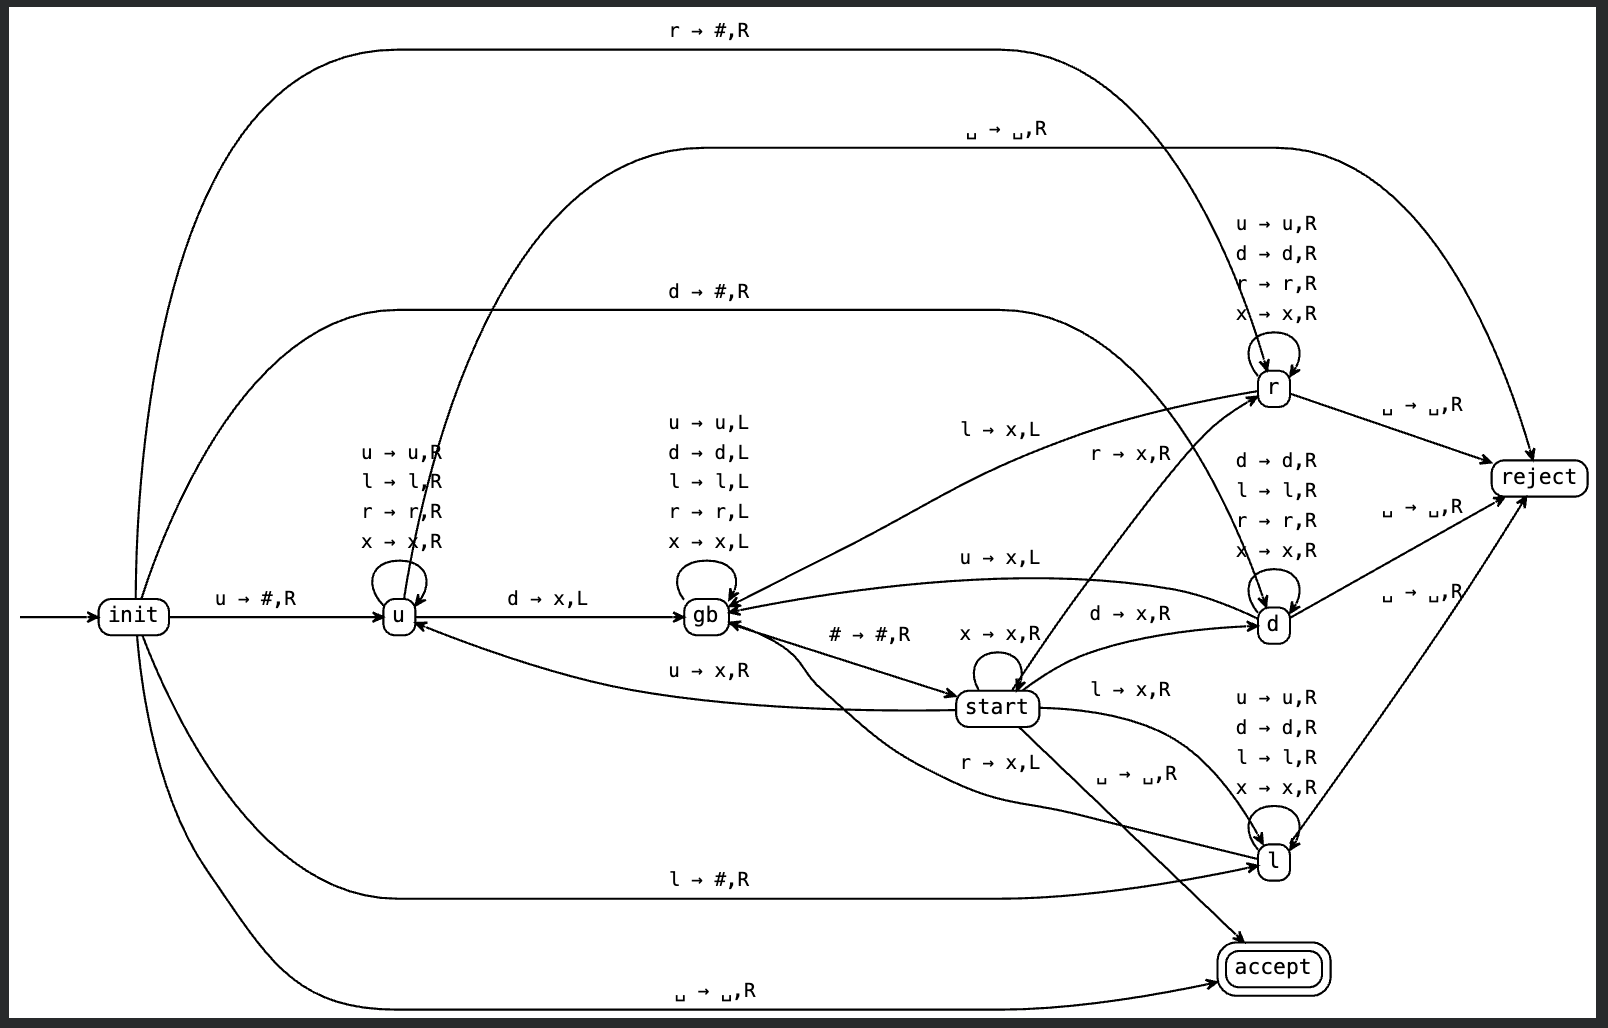
\includegraphics[width=0.75\linewidth]{p2b_tm.png}
        \end{figure}

        The CSV file for the Turing machine can be found at \url{https://gist.github.com/whgriff05/f39eafeecf4e97040af2714cfacb2af3}. 

    \end{enumerate}

    \section{Turing closure properties}

    \begin{enumerate}[(a)]
        \item Write an \textbf{implementation-level} description of a Turing machine $S$ that, on input $v \in \Sigma^*$, decides whether $v = \text{STRETCH}(u)$ for some $u$. Moreover, if $S$ accepts $v$, then when it halts, the contents of the tape should be $u$. For example, if the input is \texttt{001100}, $S$ should accept and the final contents of the tape should be \texttt{010}. But if the input is \texttt{001101}, $S$ should reject.

            $S = $ ``On input string $v$,

            \begin{enumerate}[1.]
                \item Start at the left end of the tape. If the first symbol is a blank symbol, \textit{accept}.

                \item Read the first symbol (to be referred to as the symbol being processed), change it to a blank symbol, then move the head to the right. If the next symbol is not the same as the symbol being processed, \textit{reject}.

                \item Otherwise, if it is the same, change it to a blank symbol, and move left to either the left end of the tape or the previous non-blank symbol. If on the left end, do not move. If on the previous non-blank symbol, move to the right once.

                \item Write the symbol currently being processed.

                \item Move to the right to the next non-blank symbol. If there are no more non-blank symbols, \textit{accept}. Otherwise, upon reaching the next non-blank symbol, go back to step 2."
            \end{enumerate}

        \item Prove that if $L$ is a Turing-decidable language over $\Sigma$, then STRETCH$(L)$ is also Turing-decidable. You should let $M$ be a Turing machine that decides $L$, then use your answer to 3a to give an \textbf{implementation-level} description of a Turing machine that decides STRETCH$(L)$. One of the lines of your description can be "Simulate $M$".

            If $L$ is a Turing-decidable language, that means some Turing machine $M$ decides $L$. Let another Turing machine $M'$ decide STRETCH$(L)$.

            $M' = $ ``On input string $v \in \text{STRETCH}(L)$,

            \begin{enumerate}[1.]
                \item Simulate $S$ (from Problem 3a) on $v$. If $S$ accepts, continue. Otherwise, if $S$ rejects, \textit{reject}.

                \item Move the tape left to the left end.

                \item Simulate $M$.
            \end{enumerate}

            Since the Turing machine $S$ from Problem 3a only accepts strings of the form STRETCH$(v)$ and converts the tape to $v$, any accepted stretched string will be converted to its pre-stretched form starting at the left end of the tape when $S$ accepts. Then, starting back from the left end, $M$ will decide on $v$. Since $S$ transmutes a stretched string into its original form, and $M$ can decide on the original string, STRETCH$(L)$ is Turing-decidable.

        \item Prove that if $L$ is a Turing-recognizable language, then STRETCH$(L)$ is also Turing recognizable.

            A Turing-recognizable language is defined as some Turing machine that halts and accepts strings in the language and either halts and rejects or loops on strings not in the language. Therefore, if $L$ is Turing-decidable, that is, some Turing machine halts and accepts strings in the language and halts and rejects strings not in the language, $L$ is also Turing-recognizable, as it follows the same behavior for strings in the language and one of the accepted behaviors for strings not in the language. 

            Since STRETCH$(L)$ is Turing-decidable (Problem 3b), therefore, STRETCH$(L)$ is also Turing-recognizable.
    \end{enumerate}

    
\end{document}
